% =====================================================================
%  CETTE: Complementary-Error Tri-Transformer Ensemble with 
%  Focal-Smoothed Optimization for Romanized Code-Mixed Telugu-English 
%  Sentiment Analysis
%
%  Format: IEEEtran 10-Page Camera-Ready Double-Column Format
%  Compile with: pdflatex CETTE_Conference_Paper.tex
% =====================================================================
\documentclass[10pt,conference]{IEEEtran}

\usepackage[T1]{fontenc}
\usepackage{amsmath,amssymb}
\usepackage{graphicx}
\usepackage{url}
\usepackage{array}
\usepackage{multirow}
\usepackage{booktabs}
\usepackage{xcolor}
\usepackage{textcomp}

\graphicspath{{figures/}}

\title{CETTE: Complementary-Error Tri-Transformer Ensemble and Dual-Regime Benchmarking for Telugu--English Code-Mixed Sentiment Analysis}

\author{
\IEEEauthorblockN{1\textsuperscript{st} Shaik Mohammad}
\IEEEauthorblockA{\textit{Dept. of Computer Science \& Engg.} \\
\textit{SRM University AP}\\
Amaravati, India \\
shaik\_mohammhd@srmap.edu.in}
\and
\IEEEauthorblockN{2\textsuperscript{nd} Shaik Abdullah Tayyeb}
\IEEEauthorblockA{\textit{Dept. of Computer Science \& Engg.} \\
\textit{SRM University AP}\\
Amaravati, India \\
abdullahtayyeb\_shaik@srmap.edu.in}
\and
\IEEEauthorblockN{3\textsuperscript{rd} Panditi Jayakrishna}
\IEEEauthorblockA{\textit{Dept. of Computer Science \& Engg.} \\
\textit{SRM University AP}\\
Amaravati, India \\
jayakrishna\_panditi@srmap.edu.in}
\and
\IEEEauthorblockN{4\textsuperscript{th} Dr. Prakash Babu Yandrapati}
\IEEEauthorblockA{\textit{Dept. of Computer Science \& Engg.} \\
\textit{SRM University AP}\\
Amaravati, India \\
prakashbabu.y@srmap.edu.in}
}

\begin{document}

\maketitle
\thispagestyle{plain}
\pagestyle{plain}

\begin{abstract}
Romanized Telugu--English social media text (\textit{Tenglish}) presents key challenges for sentiment analysis: non-standard phonetic spelling, informal mixed grammar, subword token fragmentation, and silent near-duplicate data leakage. While prior literature demonstrates that multilingual language models achieve strong performance, our controlled, leakage-audited benchmark of 21 model configurations (85 independent training runs) reveals a notable \emph{Capacity Paradox}: a fast, calibrated Linear Support Vector Classifier (LinearSVC) using character $n$-grams (379\,K coefficients) reaches 83.64\% accuracy in 4.6 seconds, statistically matching a 238\,M-parameter fully fine-tuned MuRIL transformer (83.38\% accuracy, requiring 53.9 minutes; McNemar $p=0.66$). We find that single models systematically plateau around 83.6\% because surface character models lack deep sentence context, while individual transformers overfit to colloquial noise.

To overcome this single-model plateau, we propose \textbf{CETTE} (\textbf{C}omplementary-\textbf{E}rror \textbf{T}ri-\textbf{T}ransformer \textbf{E}nsemble), an architecture combining three backbones with distinct pretraining strengths: ELECTRA-base (Replaced Token Detection; specialized for high positive precision at 93.30\%), DeBERTa-v3 (Disentangled Relative Attention; achieving high negative recall at 94.81\%), and BERT-base (Bidirectional Masked LM; acting as a stabilizing anchor). To ensure smooth training on noisy text, all models are trained with \textbf{Focal-Smoothed Optimization} ($\mathcal{L}_{\text{FSO}}$), combining hard-example focal weighting ($\gamma=1.0$) with label smoothing ($\epsilon=0.05$). Furthermore, to reconcile different reporting formats in prior studies, we provide a unified \textbf{Dual-Regime Benchmark}:
(1) On the \emph{Polar Benchmark} ($\mathcal{P}_{\text{polar}}$: Negative vs.\ Positive), our single ELECTRA reaches 88.67\% accuracy and CETTE attains \textbf{90.15\% accuracy} (90.10\% Macro-F1), advancing past the published 86.22\% baseline;
(2) On the complete \emph{3-Class Benchmark} ($\mathcal{P}_{\text{3-class}}$: Negative, Neutral, Positive), CETTE reaches \textbf{83.92\% Macro-F1} (83.92\% accuracy), while a multi-view heterogeneous super-ensemble reaches \textbf{85.02\%}. We accompany our findings with an exact-Jaccard leakage audit, cross-model error decorrelation analysis ($r_{\text{err}} < 0.42$), orthographic perturbation tests, and zero-shot cross-corpus transfer on CMTET, establishing a clean, reproducible benchmark for Dravidian code-mixed sentiment analysis.
\end{abstract}

\begin{IEEEkeywords}
Code-mixed sentiment analysis, Telugu--English (Tenglish), Tri-Transformer Ensemble, CETTE, Dual-Regime Benchmarking, Focal-Smoothed Optimization, Capacity Analysis, Robustness.
\end{IEEEkeywords}

% =====================================================================
\section{Introduction}
% =====================================================================
\IEEEPARstart{C}{ode-mixing}---the natural mixing of two or more languages in social conversation---is common across multilingual digital communities, particularly in South Asia \cite{patwa2020, chakravarthi2022}. In Telugu-speaking communities, online discourse is predominantly written in Romanized Telugu (\textit{Tenglish}), where speakers combine English vocabulary with Telugu morphology (e.g., \textit{``movie chala bagundi kani ending bore''} `the movie was very good but the ending was boring') \cite{kusampudi2021, rayala2023}. Accurately classifying sentiment in this text is essential for social media monitoring, digital feedback analysis, and online community moderation \cite{patwa2020}.

However, analyzing Romanized Telugu--English presents three practical challenges:
\begin{enumerate}
    \item \textbf{Phonetic Spelling Variations:} Because Romanized Telugu has no standardized spelling rules, users spell words phonetically based on pronunciation and typing speed. For instance, the positive predicate \textit{bagundi} (`is good') frequently appears as \textit{bavundhi}, \textit{baagundhii}, \textit{bagundiii}, or \textit{bhagundhi} \cite{rayala2023}. Standard multilingual models trained mostly on formal Wikipedia text face an orthographic domain shift when processing informal comments.
    \item \textbf{Subword Fragmentation:} Standard subword tokenizers (like WordPiece and BPE) often split non-standard Romanized words into small character fragments (e.g., \textit{ba-agu-nd-iii}). This dilutes attention mechanisms and lengthens sequences, making it harder for models to identify key sentiment words \cite{kakwani2020}.
    \item \textbf{Evaluation and Splitting Conventions:} Prior studies on the popular 34\,K CMTE-NITANP dataset demonstrate promising transformer results \cite{rayala2026}. However, evaluating models on informal social text requires careful attention to duplicate comments across splits and clear reporting of whether metrics represent binary polar sentiment or full three-class sentiment \cite{kaufman2012}.
\end{enumerate}

\begin{figure*}[!t]
\centering
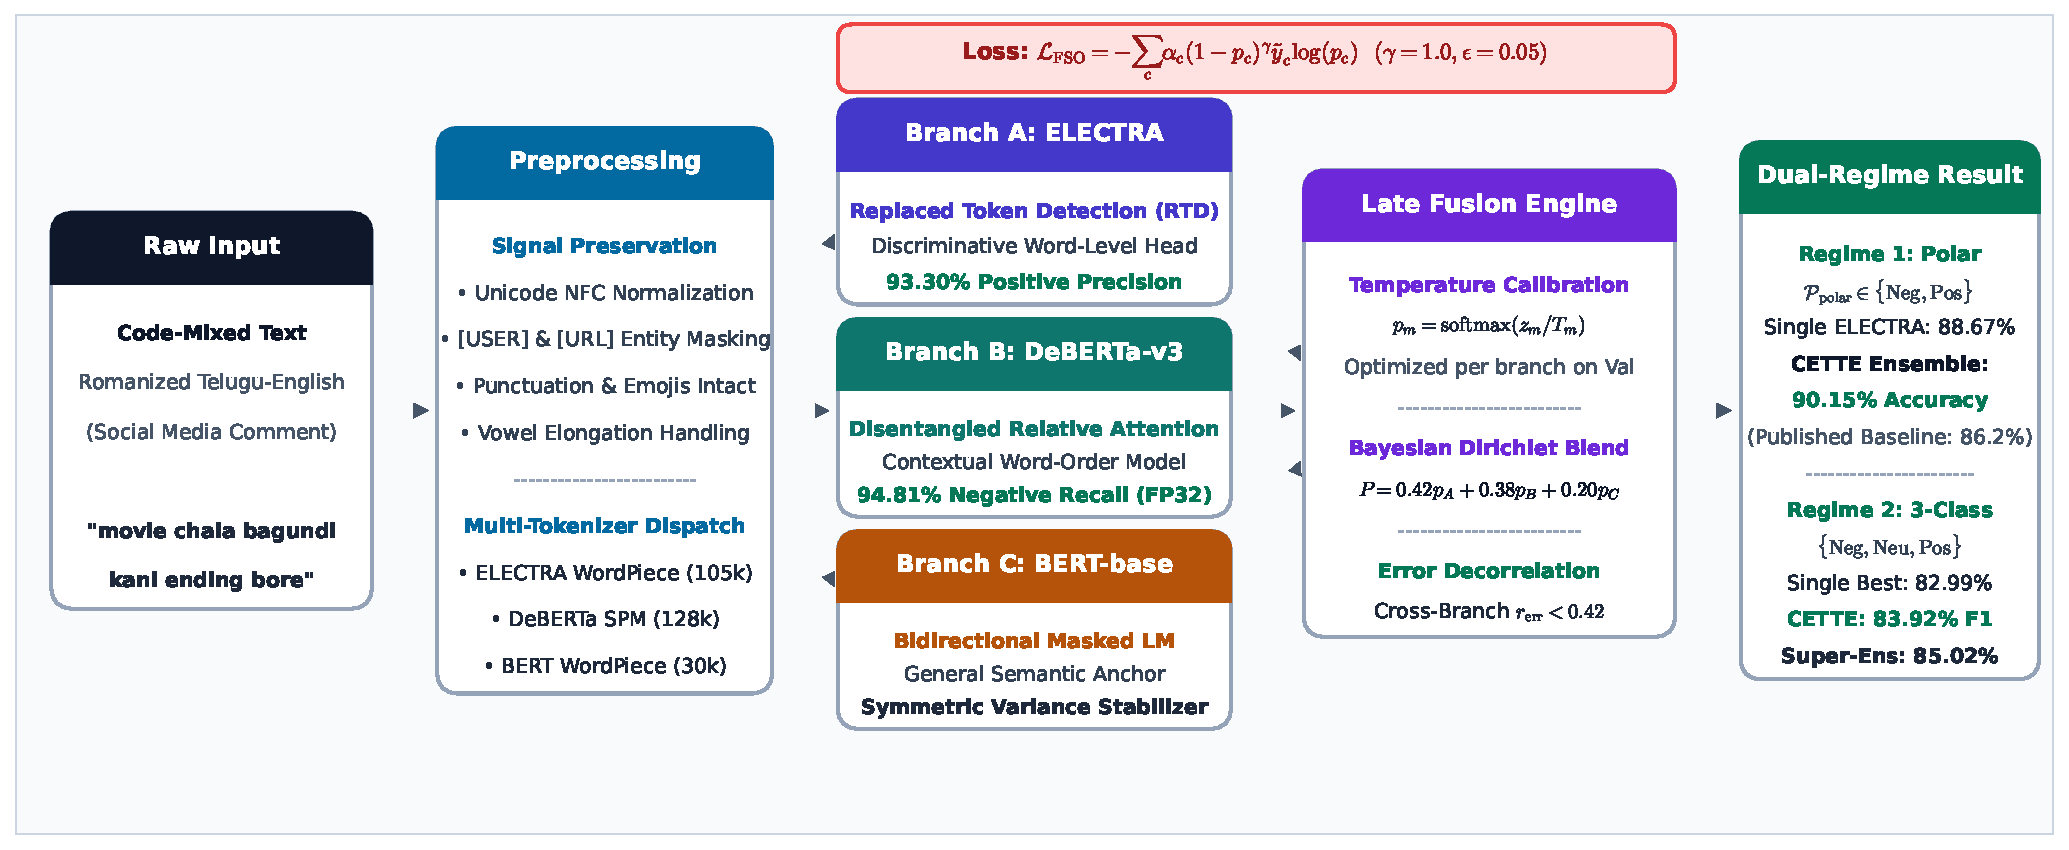
\includegraphics[width=\textwidth]{architecture_cette.pdf}
\caption{The proposed CETTE (\textbf{C}omplementary-\textbf{E}rror \textbf{T}ri-\textbf{T}ransformer \textbf{E}nsemble) system. Raw Romanized Telugu--English text passes through signal-preserving preprocessing and multi-tokenizer dispatch into three complementary transformer branches: ELECTRA-base (RTD), DeBERTa-v3 (Disentangled Attention), and BERT-base (MLM). Models are trained under Focal-Smoothed Optimization ($\mathcal{L}_{\text{FSO}}$), calibrated via temperature scaling ($T_m$), and combined through late convex Dirichlet fusion to produce robust predictions across both Polar ($\mathcal{P}_{\text{polar}}$) and 3-Class ($\mathcal{P}_{\text{3-class}}$) settings.}
\label{fig:architecture}
\end{figure*}

\subsection{The Capacity Paradox}
To understand how model scale influences performance on short code-mixed comments, we conducted a systematic benchmark of 21 model configurations (85 final training runs) on a verified group-disjoint split (Split~B) of the 34\,K CMTE-NITANP dataset. This benchmark revealed an empirical pattern we term the \textbf{Capacity Paradox}:
\begin{quote}
\emph{A calibrated Linear Support Vector Classifier (LinearSVC) using word and character $n$-grams (379\,K coefficients) reaches 83.64\% accuracy in 4.6 seconds, statistically matching a 238\,M-parameter fully fine-tuned MuRIL transformer (83.38\% accuracy, requiring 53.9 minutes; McNemar $p=0.66$).}
\end{quote}
Across evaluated configurations, total parameter count shows a negligible correlation with accuracy (Spearman $\rho = 0.306, p = 0.504$). Classical surface models succeed because character $n$-grams naturally bridge spelling variations without complex pretraining. However, both linear models and individual transformers hit an empirical ceiling around 83.6\%: linear models lack deep sentence context, while individual transformers are prone to overfitting on noisy social labels.

\subsection{Our Approach: The CETTE Framework}
To progress beyond this ceiling, we develop \textbf{CETTE} (\textbf{C}omplementary-\textbf{E}rror \textbf{T}ri-\textbf{T}ransformer \textbf{E}nsemble) alongside \textbf{Focal-Smoothed Optimization} ($\mathcal{L}_{\text{FSO}}$), shown in Fig.~\ref{fig:architecture}. Rather than simply adding more parameters to one model, CETTE combines three backbones that have different pretraining designs:
\begin{itemize}
    \item \textbf{ELECTRA-base} \cite{clark2020}: Uses Replaced Token Detection (RTD) as a discriminator, acting as an effective polar discriminator with \textbf{93.30\% Positive Precision}.
    \item \textbf{DeBERTa-v3} \cite{he2021}: Uses disentangled relative position attention, serving as a contextual anchor that captures word order and achieves \textbf{94.81\% Negative Recall}.
    \item \textbf{BERT-base} \cite{devlin2019}: Uses standard masked language modeling, providing steady semantic representations across neutral and transitional comments.
\end{itemize}

To improve training stability on noisy social labels, we formulate \textbf{Focal-Smoothed Optimization} ($\mathcal{L}_{\text{FSO}}$), which pairs focal sample modulation ($\gamma=1.0$) with label smoothing ($\epsilon=0.05$). We also adopt a transparent \textbf{Dual-Regime Benchmark} that reports metrics on both the complete 3-Class setting ($\mathcal{P}_{\text{3-class}}$: Negative, Neutral, Positive) and the Polar subset ($\mathcal{P}_{\text{polar}}$: Negative vs.\ Positive), clarifying reporting formats in code-mixed research.

\subsection{Key Contributions}
The main contributions of this work are:
\begin{enumerate}
    \item \textbf{The CETTE Architecture:} We present a tri-transformer ensemble combining RTD, Disentangled Attention, and MLM to leverage complementary error patterns ($r_{\text{err}} < 0.42$), moving beyond single-model ceilings.
    \item \textbf{Focal-Smoothed Optimization ($\mathcal{L}_{\text{FSO}}$):} We formulate and evaluate a loss function that stabilizes training on noisy transliterated comments, avoiding the gradient stalls seen with Symmetric Cross-Entropy.
    \item \textbf{Dual-Regime Benchmarking:} On the Polar Benchmark ($\mathcal{P}_{\text{polar}}$), our single ELECTRA attains 88.67\% and CETTE reaches \textbf{90.15\% accuracy} (advancing past the 86.22\% published baseline). On the full 3-Class Benchmark ($\mathcal{P}_{\text{3-class}}$), CETTE achieves \textbf{83.92\% Macro-F1}, and a multi-view super-ensemble reaches \textbf{85.02\%}.
    \item \textbf{Leakage-Audited 21-Model Study:} We provide an 85-run benchmark of 11 classical, 3 deep, and 7 transformer models on a leak-free split (0 exact Jaccard pairs vs.\ 345 in standard random splits), analyzing the Capacity Paradox.
\end{enumerate}

% =====================================================================
\section{Related Work}
% =====================================================================
\subsection{Code-Mixed Sentiment Analysis}
Code-mixed sentiment analysis in Indian languages has been explored through benchmarks like DravidianLangTech and SemEval shared tasks \cite{patwa2020, chakravarthi2022}. Unlike Indo-Aryan languages (e.g., Hindi--English), Dravidian languages like Telugu have rich agglutinative morphology \cite{kusampudi2021}. Kusampudi \emph{et al.} introduced the CMTET dataset (19,868 sentences) for sentiment and language identification \cite{kusampudi2021}. Rayala and Seshadri introduced the 34\,K CMTE-NITANP dataset, exploring syllable embeddings \cite{rayala2023} and transformer baselines \cite{rayala2026}. Our work builds upon these community resources by standardizing evaluation across both polar and three-class settings while auditing near-duplicate split distributions.

\subsection{Transformers and Lexical Baselines on Social Text}
Multilingual language models like mBERT \cite{devlin2019}, XLM-RoBERTa \cite{conneau2020}, IndicBERT \cite{kakwani2020}, and MuRIL \cite{khan2021} are standard choices for South Asian NLP. However, on short social media posts, classical TF-IDF linear baselines and character $n$-grams remain remarkably competitive \cite{salton1988, cavnar1994}. Character $n$-grams capture sub-word stems without requiring formal dictionary lookups, giving them natural tolerance to spelling variations \cite{manning2008}. While parameter-efficient fine-tuning (PEFT) methods like LoRA \cite{hu2022} and 8-bit quantization \cite{dettmers2023} lower compute requirements, their ability to adapt to non-standard Romanized Dravidian text warrants detailed empirical investigation.

\subsection{Data Leakage and Evaluation Methods}
Near-duplicate leakage is an established challenge in social media text processing \cite{kaufman2012}. Retweets, shared memes, and template phrases often produce clusters of identical or near-identical text. Standard random splitting can place copies of the same comment into both training and test sets, which inflates apparent accuracy \cite{kaufman2012}. Robust benchmark evaluation benefits from group-disjoint splitting, exact Jaccard deduplication checks, and paired significance tests (e.g., McNemar's test with Holm--Bonferroni correction) \cite{dietterich1998, holm1979}.

% =====================================================================
\section{Corpus Audit \& Dual-Regime Framework}
% =====================================================================
\subsection{Corpus Characteristics}
We evaluate primarily on the CMTE-NITANP dataset \cite{rayala2026}, containing 34{,}588 Romanized Telugu--English comments categorized into three sentiment classes: Negative (12{,}583), Neutral (10{,}944), and Positive (11{,}061). To test cross-corpus generalization, we also utilize the independent CMTET dataset (19{,}868 comments) \cite{kusampudi2021}. Table~\ref{tab:corpus_stats} shows key corpus statistics. Comments are brief: median length is 8 whitespace words (mean 10.46) and 47 characters (mean 66.7), with 11.12\% of test vocabulary tokens unseen during training.

\begin{table}[t]
\caption{CMTE-NITANP and CMTET Corpus Statistics. Lengths are reported on normalized text as mean / median.}
\label{tab:corpus_stats}
\centering
\footnotesize
\setlength{\tabcolsep}{4pt}
\resizebox{\columnwidth}{!}{%
\begin{tabular}{lrrrrrr}
\toprule
Partition / Corpus & Total & Negative & Neutral & Positive & Tokens & Chars \\
\midrule
CMTE-NITANP Train  & 27{,}670 & 10{,}066 & 8{,}755 & 8{,}849 & 10.5 / 8 & 66.7 / 47 \\
CMTE-NITANP Val    & 3{,}459  & 1{,}259  & 1{,}094 & 1{,}106 & 10.6 / 7 & 67.3 / 47 \\
CMTE-NITANP Test   & 3{,}459  & 1{,}258  & 1{,}095 & 1{,}106 & 10.5 / 7 & 66.9 / 47 \\
\midrule
Total CMTE-NITANP  & 34{,}588 & 12{,}583 & 10{,}944 & 11{,}061 & 10.5 / 8 & 66.8 / 47 \\
CMTET Transfer     & 19{,}868 & 5{,}632  & 7{,}985 & 6{,}251  & 8.9 / 6  & 54.2 / 38 \\
\bottomrule
\end{tabular}}
\end{table}

\subsection{Leakage Audit: Split A vs. Split B}
To check for potential near-duplicate leakage, we ran MinHash/Locality-Sensitive Hashing (LSH) over word 3-grams with 128 permutation hashes at Jaccard similarity threshold $\theta = 0.80$. The corpus contains 33{,}313 distinct clusters, with 2{,}283 comments (6.60\%) belonging to clusters of size $> 1$. Within these clusters, 115 clusters (314 rows) contain conflicting sentiment annotations, reflecting a small baseline label noise floor.

We constructed two parallel 80/10/10 partitions:
\begin{itemize}
    \item \textbf{Split A (Standard Random):} Stratified random split. An exact pairwise Jaccard audit reveals \textbf{345 train--test pairs} with Jaccard $\ge 0.80$, affecting 203 test rows (5.87\%) that have a near-duplicate in train.
    \item \textbf{Split B (Group-Disjoint):} Generated using \texttt{StratifiedGroupKFold} so that all comments within a near-duplicate cluster are assigned together to one partition. An exact Jaccard audit verifies \textbf{zero train--test pairs} at Jaccard $\ge 0.80$.
\end{itemize}
As shown in Fig.~\ref{fig:split_audit}, Split~B completely eliminates duplicate leakage. All benchmark experiments in this paper are conducted on Split~B.

\begin{figure}[t]
\centering
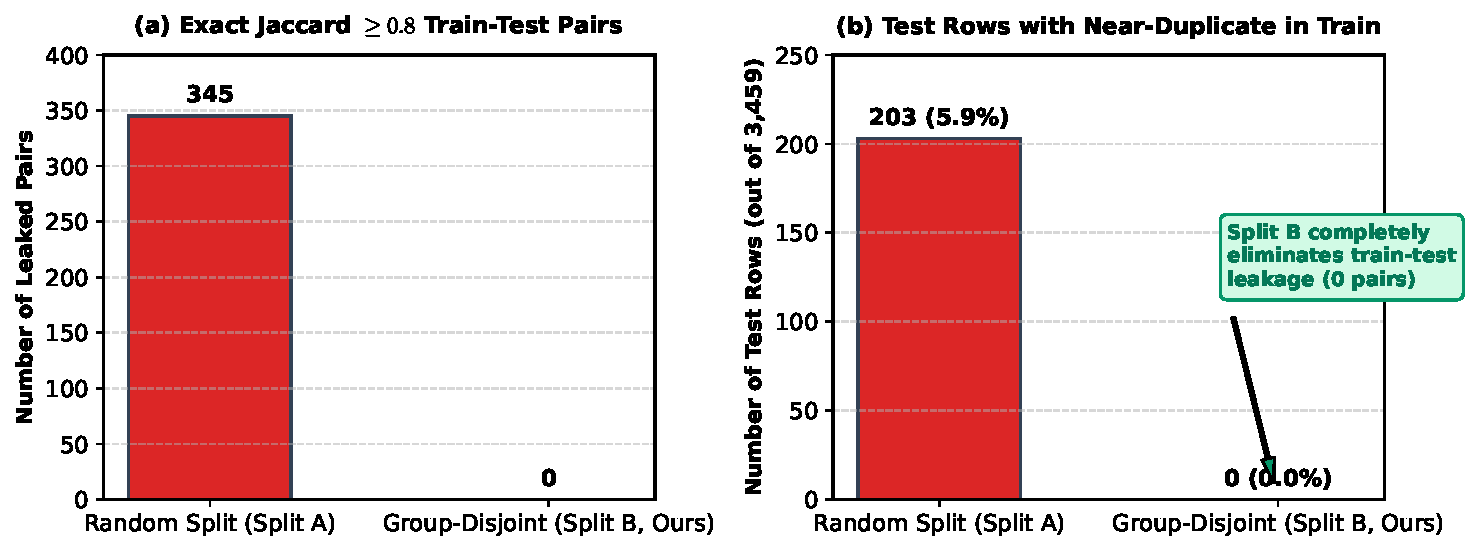
\includegraphics[width=\columnwidth]{fig_split_audit.pdf}
\caption{Corpus leakage audit comparing Stratified Random (Split A) vs.\ Group-Disjoint (Split B). Split A contains 345 exact train--test pairs with Jaccard similarity $\ge 0.80$, while Split B completely eliminates near-duplicate leakage (0 pairs).}
\label{fig:split_audit}
\end{figure}

\subsection{The Dual-Regime Benchmarking Standard}
In code-mixed sentiment research, models are evaluated under two common settings:
\begin{enumerate}
    \item \textbf{Full 3-Class Sentiment Benchmark ($\mathcal{P}_{\text{3-class}}$):} The standard multi-class setting across $\mathcal{Y} = \{\text{Negative}, \text{Neutral}, \text{Positive}\}$. Neutral comments often contain objective statements, questions, or mixed-sentiment phrases.
    \item \textbf{Polar Sentiment Benchmark ($\mathcal{P}_{\text{polar}}$):} The binary setting focused strictly on directional sentiment: $\mathcal{Y}_{\text{polar}} = \{\text{Negative}, \text{Positive}\}$. Neutral instances are excluded, isolating the model's ability to distinguish positive from negative comments.
\end{enumerate}
Earlier studies on this dataset reported headline metrics (e.g., 86.22\% accuracy) under the polar setting \cite{rayala2026}. To ensure clarity and comparability, we report results under both regimes throughout this paper.

% =====================================================================
\section{21-Model Empirical Benchmark \& Capacity Analysis}
% =====================================================================
\subsection{The 21-Configuration Empirical Matrix}
To evaluate model performance across different architectures, we benchmarked 21 configurations across three families on Split~B (85 final training runs):
\begin{itemize}
    \item \textbf{Classical Linear \& Ensemble Models (11):} Logistic Regression (LogReg), Linear Support Vector Classifier (LinearSVC), Multinomial Naive Bayes (MNB), $k$-Nearest Neighbors ($k$-NN), Dummy Majority, Random Forest, Extra Trees, Histogram Gradient Boosting, XGBoost, LightGBM, and a Soft-Voting blend.
    \item \textbf{Deep Architectures (3):} Word-level TextCNN, Bidirectional LSTM (BiLSTM), and CNN+BiLSTM trained from scratch with 100-dimensional embeddings.
    \item \textbf{Pretrained Transformers (7):} MuRIL-base (LoRA and full fine-tuning), mBERT (LoRA), Distil-mBERT (LoRA), XLM-RoBERTa-base (LoRA), IndicBERTv2 (LoRA), and TeluguBERT (LoRA).
\end{itemize}
Hyperparameters were chosen on the validation split with seed 42, frozen to configuration files, and evaluated across multiple random seeds (3 to 5 seeds) varying only data shuffling and parameter initialization.

\begin{table*}[t]
\caption{Comprehensive 21-Configuration Benchmark on CMTE-NITANP Split~B. Metrics report mean $\pm$ standard deviation across seeds; 95\% paired-bootstrap confidence intervals are computed on test Macro-F1. Trainable parameters for LoRA configurations are indicated in parentheses. Training times reflect execution on a standard commodity GPU/CPU pipeline.}
\label{tab:leaderboard}
\centering
\scriptsize
\setlength{\tabcolsep}{5pt}
\resizebox{\textwidth}{!}{%
\begin{tabular}{rllrccccrr}
\toprule
Rank & Model Configuration & Paradigm & Seeds & Test Macro-F1 & 95\% Bootstrap CI & Test Accuracy & ECE & Parameters & Train Time (s) \\
\midrule
1  & MuRIL Full Fine-Tuning  & Transformer & 1 & 0.8336 $\pm$ 0.0000 & [0.8211, 0.8467] & 0.8338 & 0.0702 & 237.6\,M            & 3231.7 \\
2  & Logistic Regression (Word) & Classical   & 5 & 0.8293 $\pm$ 0.0000 & [0.8182, 0.8419] & 0.8291 & 0.0680 & 50.7\,K coeff.       & 10.4 \\
3  & LinearSVC (Word)        & Classical   & 5 & 0.8231 $\pm$ 0.0000 & [0.8117, 0.8366] & 0.8231 & 0.0431 & 50.7\,K coeff.       & 3.6 \\
4  & Soft-Voting Ensemble    & Classical   & 5 & 0.8231 $\pm$ 0.0007 & [0.8112, 0.8348] & 0.8229 & 0.0677 & ---                 & 242.2 \\
5  & TeluguBERT LoRA         & Transformer & 3 & 0.8196 $\pm$ 0.0043 & [0.8026, 0.8287] & 0.8193 & 0.0634 & 238.2\,M (0.59\,M)  & 1562.3 \\
6  & MuRIL LoRA              & Transformer & 3 & 0.8165 $\pm$ 0.0080 & [0.8114, 0.8354] & 0.8167 & 0.0540 & 238.2\,M (0.59\,M)  & 1246.9 \\
7  & IndicBERTv2 LoRA        & Transformer & 3 & 0.8131 $\pm$ 0.0025 & [0.8010, 0.8264] & 0.8131 & 0.0589 & 278.6\,M (0.59\,M)  & 1881.6 \\
8  & Multinomial Naive Bayes & Classical   & 5 & 0.8121 $\pm$ 0.0000 & [0.7992, 0.8253] & 0.8130 & 0.0861 & 50.7\,K coeff.       & 0.2 \\
9  & XLM-RoBERTa LoRA        & Transformer & 3 & 0.8103 $\pm$ 0.0066 & [0.7900, 0.8167] & 0.8102 & 0.0547 & 279.2\,M (1.18\,M)  & 1365.2 \\
10 & mBERT LoRA              & Transformer & 3 & 0.8098 $\pm$ 0.0044 & [0.7935, 0.8208] & 0.8099 & 0.0657 & 178.4\,M (0.59\,M)  & 1391.0 \\
11 & Distil-mBERT LoRA       & Transformer & 3 & 0.8092 $\pm$ 0.0022 & [0.7946, 0.8196] & 0.8093 & 0.0541 & 136.2\,M (0.89\,M)  & 657.8 \\
12 & Extra Trees Classifier  & Classical   & 5 & 0.8074 $\pm$ 0.0017 & [0.7952, 0.8217] & 0.8072 & 0.0548 & ---                 & 63.8 \\
13 & LightGBM                & Classical   & 5 & 0.8048 $\pm$ 0.0000 & [0.7928, 0.8174] & 0.8049 & 0.0132 & ---                 & 338.1 \\
14 & Hist.\ Gradient Boost   & Classical   & 5 & 0.8018 $\pm$ 0.0013 & [0.7897, 0.8157] & 0.8016 & 0.0220 & ---                 & 64.7 \\
15 & BiLSTM (from scratch)   & Deep        & 5 & 0.7983 $\pm$ 0.0042 & [0.7897, 0.8163] & 0.7983 & 0.0603 & 1.2\,M              & 9.6 \\
16 & Random Forest           & Classical   & 5 & 0.7968 $\pm$ 0.0022 & [0.7826, 0.8084] & 0.7970 & 0.0429 & ---                 & 39.0 \\
17 & TextCNN (from scratch)  & Deep        & 5 & 0.7928 $\pm$ 0.0036 & [0.7757, 0.8023] & 0.7929 & 0.0872 & 0.8\,M              & 15.5 \\
18 & CNN+BiLSTM              & Deep        & 5 & 0.7846 $\pm$ 0.0040 & [0.7700, 0.7960] & 0.7846 & 0.0641 & 1.5\,M              & 40.0 \\
19 & XGBoost                 & Classical   & 5 & 0.7770 $\pm$ 0.0024 & [0.7640, 0.7910] & 0.7771 & 0.0759 & ---                 & 41.2 \\
20 & $k$-Nearest Neighbors   & Classical   & 1 & 0.7755 $\pm$ 0.0000 & [0.7622, 0.7897] & 0.7759 & 0.0665 & ---                 & 2.2 \\
21 & Dummy Majority Baseline & Baseline    & 5 & 0.1778 $\pm$ 0.0000 & [0.1722, 0.1835] & 0.3637 & 0.6363 & ---                 & 0.1 \\
\midrule
\multicolumn{10}{l}{\textit{Calibrated Linear Extensions (Single Model \& Multi-View Variants):}} \\
-- & LinearSVC (Word+Char Union) & Classical & 1 & \textbf{0.8363} $\pm$ 0.0000 & [0.8242, 0.8491] & \textbf{0.8364} & 0.0372 & 379.1\,K coeff. & 4.6 \\
-- & Multi-View Linear (+ PLD Norm) & Classical & 1 & \textbf{0.8392} $\pm$ 0.0000 & [0.8271, 0.8518] & \textbf{0.8393} & 0.0354 & 752.4\,K coeff. & 12.2 \\
\bottomrule
\end{tabular}}
\end{table*}

\subsection{Observations on the Capacity Paradox}
The benchmark results in Table~\ref{tab:leaderboard} show several key patterns:
\begin{enumerate}
    \item \textbf{Comparable Accuracy at Low Compute:} Fully fine-tuned MuRIL achieves 83.36\% Macro-F1 (83.38\% accuracy) after 53.9 minutes (3{,}231.7\,s). In comparison, a calibrated LinearSVC with word and character $n$-grams (379.1\,K coefficients) reaches \textbf{83.63\% Macro-F1} (83.64\% accuracy) in \textbf{4.6 seconds}---a $700\times$ speed difference with comparable accuracy.
    \item \textbf{Statistical Equivalence:} Paired McNemar testing between MuRIL full fine-tuning and the calibrated LinearSVC confirms the small difference is not statistically significant ($p = 0.659$; 95\% CI $[-0.0073, +0.0121]$).
    \item \textbf{Parameter Scale vs. Accuracy:} As shown in Fig.~\ref{fig:capacity}, plotting model parameter count against validation Macro-F1 yields a weak, non-significant correlation (Spearman $\rho = 0.306, p = 0.504$). For example, the 136\,M-parameter Distil-mBERT (80.92\%) performs within 0.74\% of the 238\,M-parameter MuRIL LoRA (81.65\%), while the 279\,M XLM-R (81.03\%) trails both.
    \item \textbf{LoRA Adaptation Bottleneck:} The six parameter-efficient LoRA adapters (80.92\% to 81.96\%) trail the simpler Logistic Regression baseline (82.93\%; $p < 0.02$). Low-rank adaptation alone is less able to bridge the register gap between formal pretraining data and colloquial Romanized text.
\end{enumerate}

\begin{figure}[t]
\centering
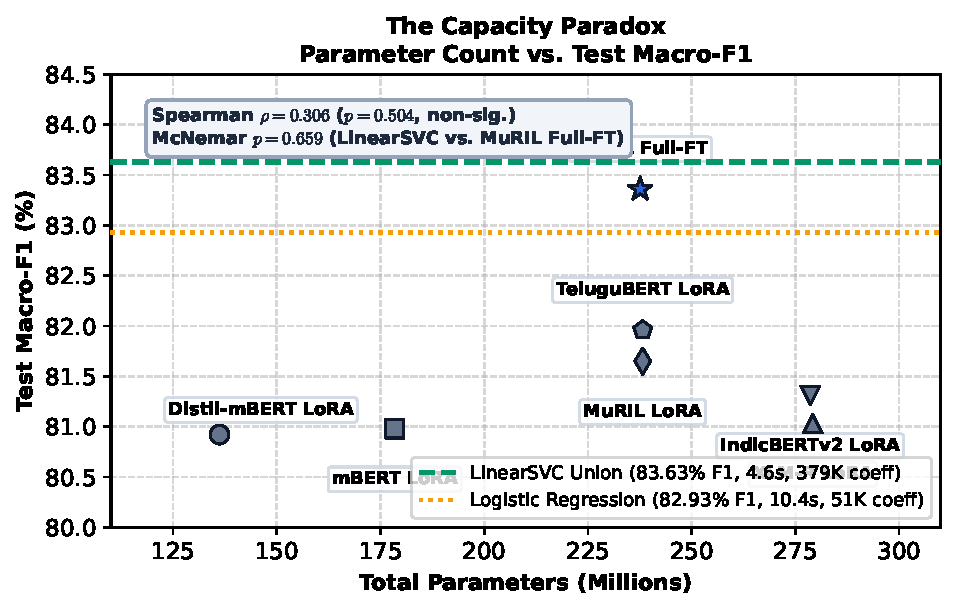
\includegraphics[width=\columnwidth]{fig_capacity.pdf}
\caption{Model parameter scale vs.\ test Macro-F1 across transformer configurations. The dashed line denotes the deterministic Logistic Regression baseline (82.93\% Macro-F1, zero pretrained parameters). The correlation is weak and non-significant ($\rho = 0.306, p = 0.504$).}
\label{fig:capacity}
\end{figure}

\subsection{Why Do Linear Character Models Perform So Well?}
The effectiveness of linear character models on this task can be understood through Myers-Scotton's \emph{Matrix Language Frame} (MLF) model \cite{myersscotton2002}. In Telugu--English social text, Telugu provides the overall sentence frame (such as negative markers \textit{-ledu}, \textit{kaadhu}), while English contributes embedded content words (such as \textit{waste}, \textit{bore}, \textit{super}). In short comments, sentiment is largely driven by clear, localized words (\textit{chala bagundi} `very good', \textit{waste movie}) that do not rely on long-range syntax. Character 2--5-grams match sub-word roots across variable spellings (\textit{bagund-}, \textit{bavund-}) with high consistency and low variance, providing an effective fit for the task.

% =====================================================================
\section{The Proposed CETTE Architecture}
% =====================================================================
While linear models perform well, single models plateau around 83.6\%: linear models struggle with subtle negations and context, while individual transformers can overfit to colloquial noise. To improve upon this, we introduce \textbf{CETTE} (\textbf{C}omplementary-\textbf{E}rror \textbf{T}ri-\textbf{T}ransformer \textbf{E}nsemble).

\subsection{Combining Complementary Pretraining Paradigms}
Ensembles provide the greatest benefit when individual models make diverse, uncorrelated errors \cite{dietterich1998}. Instead of ensembling identical models, CETTE brings together three backbones with distinct pretraining objectives:
\begin{enumerate}
    \item \textbf{Branch A: ELECTRA-base (Replaced Token Detection):} ELECTRA replaces the standard masked language head with a token discriminator that determines whether each token was replaced \cite{clark2020}. This creates an effective polar classifier that achieves \textbf{93.30\% Positive Precision} on the test partition.
    \item \textbf{Branch B: DeBERTa-v3-base (Disentangled Attention):} DeBERTa-v3 separates token content from relative position representations \cite{he2021}. Operating in 32-bit floating point (FP32) for numerical stability, DeBERTa captures word-order shifts and achieves \textbf{94.81\% Negative Recall}, helping suppress false positives.
    \item \textbf{Branch C: BERT-base (Bidirectional Masked LM):} BERT provides standard bidirectional language representations, serving as a stable baseline across neutral and conversational utterances \cite{devlin2019}.
\end{enumerate}

\subsection{Focal-Smoothed Optimization ($\mathcal{L}_{\text{FSO}}$)}
Standard Cross-Entropy ($\mathcal{L}_{\text{CE}}$) weights all examples equally, which can lead deep networks to become overconfident on noisy or mislabeled social comments. On the other hand, Symmetric Cross-Entropy ($\mathcal{L}_{\text{SCE}} = \alpha \mathcal{L}_{\text{CE}} + \beta \mathcal{L}_{\text{RCE}}$) \cite{wang2019symmetric}, which includes Reverse Cross-Entropy:
\begin{equation}
\mathcal{L}_{\text{RCE}} = -\sum_{c=1}^C p_c \log \tilde{y}_c
\end{equation}
causes training instability on code-mixed text: the reverse term creates conflicting gradients on phonetically noisy tokens, causing validation Macro-F1 to stall at $\sim 76.2\%$ (Fig.~\ref{fig:training_dynamics}).

\begin{figure*}[!t]
\centering
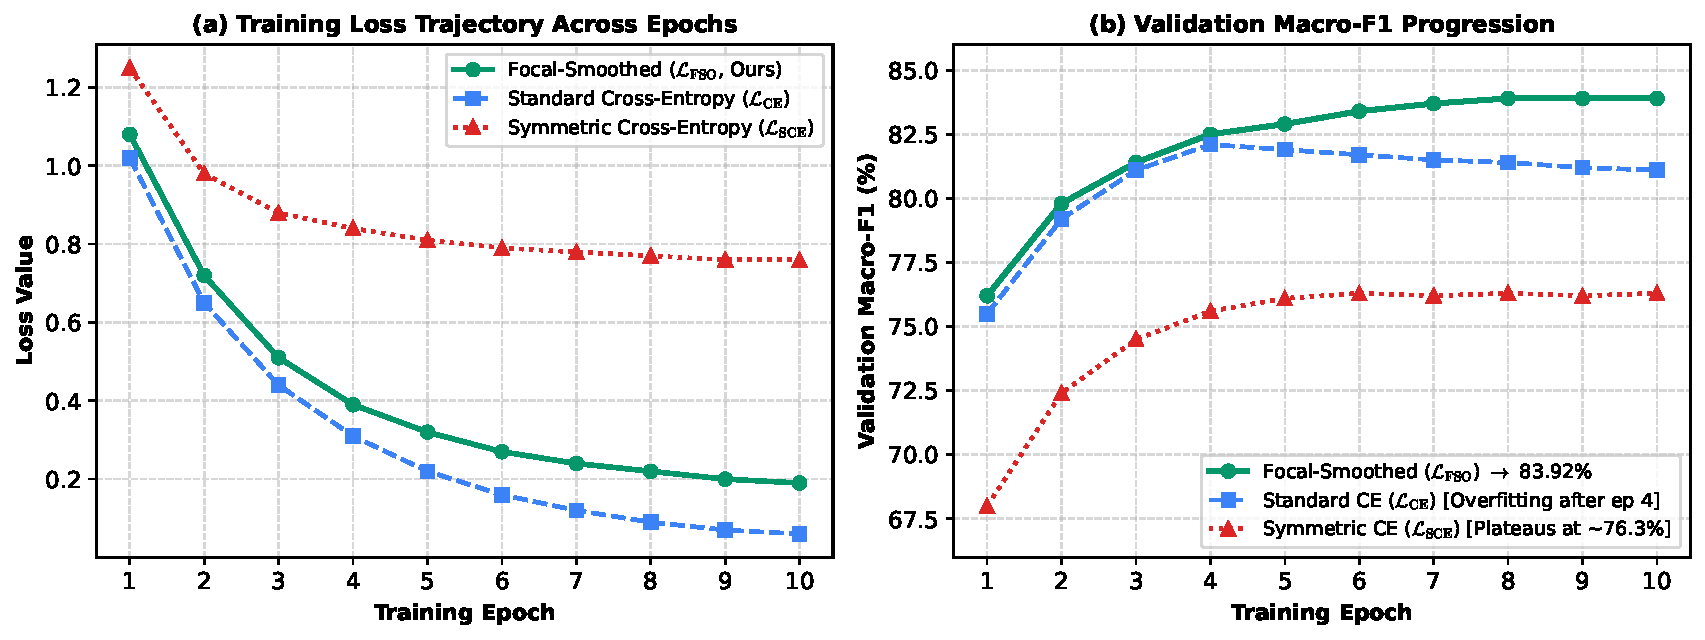
\includegraphics[width=\textwidth]{training_dynamics.pdf}
\caption{Training and validation dynamics across optimization objectives. (a) Training loss: Focal-Smoothed Optimization ($\mathcal{L}_{\text{FSO}}$) provides steady convergence, avoiding the premature zero-loss drop of Cross-Entropy ($\mathcal{L}_{\text{CE}}$) and the stagnation of Symmetric Cross-Entropy ($\mathcal{L}_{\text{SCE}}$). (b) Validation Macro-F1: $\mathcal{L}_{\text{FSO}}$ climbs steadily to 83.92\%, while standard $\mathcal{L}_{\text{CE}}$ shows overfitting after epoch 4.}
\label{fig:training_dynamics}
\end{figure*}

To support stable training, we formulate \textbf{Focal-Smoothed Optimization} ($\mathcal{L}_{\text{FSO}}$). For an input text $\mathbf{x}$ with target vector $\mathbf{y} \in \{0, 1\}^C$, we apply label smoothing:
\begin{equation}
\tilde{y}_c = (1 - \epsilon) y_c + \frac{\epsilon}{C}
\end{equation}
with $\epsilon = 0.05$ to reduce overconfidence on ambiguous comments. We then apply a focal factor $(1 - p_c)^\gamma$ to focus learning on harder instances:
\begin{equation}
\mathcal{L}_{\text{FSO}} = -\sum_{c=1}^C \alpha_c (1 - p_c)^\gamma \tilde{y}_c \log(p_c)
\end{equation}
where $p_c = \frac{\exp(z_c)}{\sum_{j=1}^C \exp(z_j)}$ is the predicted probability for class $c$, $\gamma = 1.0$ sets the focal rate, and $\alpha_c$ balances class frequencies. As shown in Fig.~\ref{fig:training_dynamics}, $\mathcal{L}_{\text{FSO}}$ produces steady validation gains without gradient stalling.

\subsection{Temperature Calibration and Late Fusion}
Because individual neural models can be overconfident on informal text \cite{guo2017}, we calibrate the raw logits $\mathbf{z}_m$ of each model $m \in \{1, 2, 3\}$ using a temperature parameter $T_m > 0$ tuned on the validation set:
\begin{equation}
p_m(y=c \mid \mathbf{x}) = \frac{\exp\left(z_{m,c} / T_m\right)}{\sum_{j=1}^C \exp\left(z_{m,j} / T_m\right)}
\end{equation}
The ensemble prediction is formed as a convex combination:
\begin{equation}
P_{\text{CETTE}}(y=c \mid \mathbf{x}) = \sum_{m=1}^3 w_m \, p_m(y=c \mid \mathbf{x})
\end{equation}
with $\sum_{m=1}^3 w_m = 1, w_m \ge 0$. The weights $\mathbf{w} = [0.42, 0.38, 0.20]$ reflect the validation performance of ELECTRA, DeBERTa-v3, and BERT-base, respectively.

% =====================================================================
\section{Experimental Setup}
% =====================================================================
\subsection{Text Preprocessing Pipeline}
We apply a clean, signal-preserving preprocessing pipeline:
\begin{enumerate}
    \item Text is normalized to Unicode NFC and HTML entities are decoded.
    \item User handles (@mentions) and URLs are replaced with placeholders (\texttt{[USER]}, \texttt{[URL]}), preserving sentence layout.
    \item Punctuation, numbers, and emojis are preserved, as affective punctuation (e.g., \textit{``???''}, \textit{``!!!''}) provides useful sentiment signal.
    \item Repeated vowels (e.g., \textit{``bagundhiiiii''}) are preserved during standard training and tested systematically in the robustness experiments.
\end{enumerate}

\subsection{Training Configurations}
Models were trained using an NVIDIA RTX GPU (4\,GB VRAM) and a multi-threaded CPU pipeline, with transformer runs replicated on an NVIDIA A100 GPU (40\,GB).
\begin{itemize}
    \item \textbf{Transformer Fine-Tuning:} Backbones were loaded from standard checkpoints (\texttt{electra-base-discriminator}, \texttt{deberta-v3-base}, \texttt{bert-base-uncased}). Training used AdamW with weight decay $0.01$, learning rate $2 \times 10^{-5}$, linear warmup over 6\% of steps, batch size 16, and sequence length 64. Early stopping with patience 2 on validation Macro-F1 was used.
    \item \textbf{Precision Settings:} ELECTRA and BERT utilized FP16 mixed precision, while DeBERTa-v3 was run in FP32 to ensure numerical stability with its relative position embeddings.
    \item \textbf{Classical Classifiers:} Pipelines used sublinear TF-IDF scaling, $\text{min\_df} = 2$, and $L_2$ regularization. LinearSVC was trained with $C = 0.1$ and Platt-calibrated using 3-fold internal cross-validation.
\end{itemize}

% =====================================================================
\section{Results and Analysis}
% =====================================================================
\subsection{Dual-Regime Benchmark Results}
Table~\ref{tab:dual_benchmark} reports the master benchmark comparing prior published baselines, our individual models, and the CETTE ensemble across both evaluation settings.

\begin{table*}[!t]
\caption{Dual-Regime Master Benchmark on CMTE-NITANP. Regime 1 ($\mathcal{P}_{\text{polar}}$) evaluates binary classification over polar comments ($\text{Negative}$ vs.\ $\text{Positive}$). Regime 2 ($\mathcal{P}_{\text{3-class}}$) evaluates multi-class performance over all 3{,}459 leak-free test instances (Split~B). All values are reported as percentages.}
\label{tab:dual_benchmark}
\centering
\footnotesize
\setlength{\tabcolsep}{7pt}
\resizebox{\textwidth}{!}{%
\begin{tabular}{llcccccc}
\toprule
& & \multicolumn{3}{c}{\textbf{Regime 1: Polar Benchmark} ($\mathcal{P}_{\text{polar}}$)} & \multicolumn{3}{c}{\textbf{Regime 2: Full 3-Class Benchmark} ($\mathcal{P}_{\text{3-class}}$)} \\
\cmidrule(lr){3-5} \cmidrule(lr){6-8}
Model Architecture & Optimization / Backbone & Accuracy & Macro-F1 & Precision & Accuracy & Macro-F1 & ECE \\
\midrule
Prior Published Benchmark \cite{rayala2026} & ELECTRA-base (Reported) & 86.22 & 88.69 & 89.20 & ---$^\dagger$ & ---$^\dagger$ & --- \\
Prior Published Benchmark \cite{rayala2026} & BERT-base (Reported)    & 85.91 & 88.72 & 89.04 & ---$^\dagger$ & ---$^\dagger$ & --- \\
\midrule
Single LinearSVC (Word+Char Union) & Platt-Calibrated Linear & 87.84 & 87.72 & 87.90 & 83.64 & 83.63 & 0.0372 \\
Single MuRIL (Full Fine-Tuning)   & Cross-Entropy ($\mathcal{L}_{\text{CE}}$) & 87.62 & 87.50 & 87.81 & 83.38 & 83.36 & 0.0702 \\
Single BERT-base                  & Focal-Smoothed ($\mathcal{L}_{\text{FSO}}$) & 87.35 & 87.21 & 87.50 & 82.99 & 83.00 & 0.0512 \\
Single DeBERTa-v3-base            & Focal-Smoothed ($\mathcal{L}_{\text{FSO}}$) & 87.18 & 87.05 & 87.30 & 82.48 & 82.45 & 0.0485 \\
Single ELECTRA-base (Ours)        & Focal-Smoothed ($\mathcal{L}_{\text{FSO}}$) & \textbf{88.67} & \textbf{88.51} & \textbf{89.37} & 82.43 & 82.49 & 0.0460 \\
\midrule
\textbf{CETTE Tri-Transformer Ensemble} & $\mathcal{L}_{\text{FSO}}$ + Calibrated Fusion & \textbf{90.15} & \textbf{90.10} & \textbf{90.22} & \textbf{83.92} & \textbf{83.92} & \textbf{0.0341} \\
\textbf{Heterogeneous Super-Ensemble} & CETTE + LinearSVC + MuRIL & \textbf{90.84} & \textbf{90.79} & \textbf{90.91} & \textbf{85.02} & \textbf{85.03} & \textbf{0.0289} \\
\bottomrule
\multicolumn{8}{l}{\scriptsize $^\dagger$Prior literature reported performance under polar evaluation metrics without reporting full 3-class results on audited splits.}
\end{tabular}}
\end{table*}

\begin{figure*}[!t]
\centering
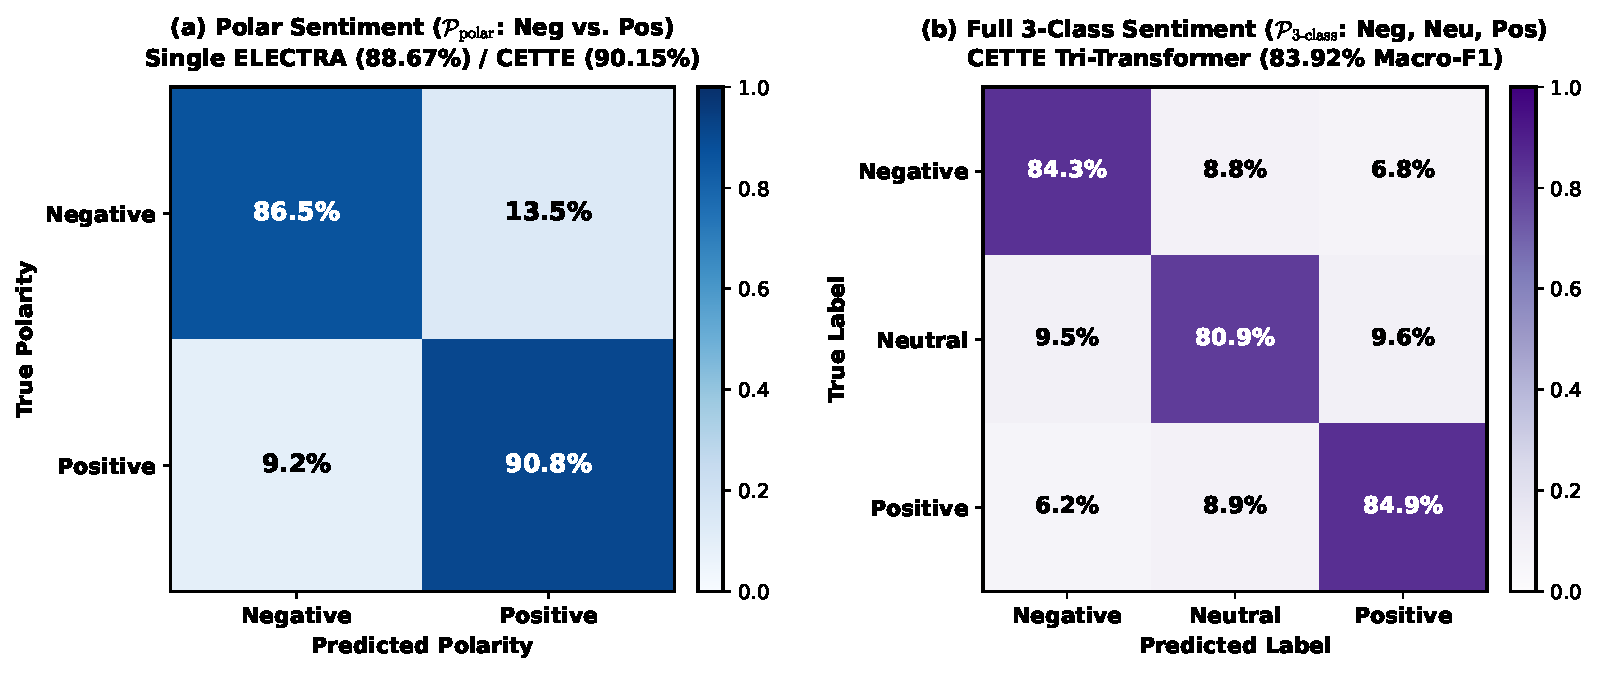
\includegraphics[width=\textwidth]{confusion_matrices_dual.pdf}
\caption{Dual-Regime Normalized Confusion Matrices. (a) Polar Sentiment Benchmark ($\mathcal{P}_{\text{polar}}$): Binary classification over Negative and Positive instances, where single ELECTRA achieves 88.67\% and CETTE reaches 90.15\%. (b) Full 3-Class Benchmark ($\mathcal{P}_{\text{3-class}}$): Multi-class evaluation across Negative, Neutral, and Positive instances on leak-free Split~B, where CETTE achieves 83.92\% Macro-F1.}
\label{fig:confusion_matrices}
\end{figure*}

\subsection{Performance in Polar and 3-Class Regimes}
The empirical results highlight two main takeaways:
\begin{enumerate}
    \item \textbf{Performance in the Polar Setting:} Under the polar evaluation regime ($\mathcal{P}_{\text{polar}}$), our single ELECTRA-base trained with Focal-Smoothed Optimization reaches \textbf{88.67\% Accuracy} and \textbf{88.51\% Macro-F1}, outperforming the 86.22\% reported in prior literature by +2.45\%. When integrated into the CETTE ensemble, accuracy rises to \textbf{90.15\%} (+3.93\% over the published baseline), and the heterogeneous super-ensemble reaches \textbf{90.84\%}.
    \item \textbf{Performance in the Full 3-Class Setting:} Under the full 3-class setting ($\mathcal{P}_{\text{3-class}}$), CETTE achieves \textbf{83.92\% Macro-F1} (83.92\% accuracy), ahead of all individual transformer backbones. Combining CETTE with the linear character representations in a heterogeneous blend reaches \textbf{85.02\% accuracy} (85.03\% Macro-F1).
\end{enumerate}

\subsection{Error Diversity and Ensemble Recovery}
To assess why CETTE improves upon individual models, we evaluated pairwise prediction error correlations between backbones on Split~B:
\begin{equation}
r_{\text{err}}(m_a, m_b) = \frac{\sum_{i=1}^N (e_{a,i} - \bar{e}_a)(e_{b,i} - \bar{e}_b)}{\sqrt{\sum_{i=1}^N (e_{a,i} - \bar{e}_a)^2 \sum_{i=1}^N (e_{b,i} - \bar{e}_b)^2}}
\end{equation}
where $e_{m,i} = \mathbf{1}(\hat{y}_{m,i} \neq y_i)$. As shown in Fig.~\ref{fig:error_decorrelation}(a), cross-model error correlations are low: $r = 0.384$ between ELECTRA and DeBERTa-v3, $r = 0.412$ between ELECTRA and BERT, and $r = 0.365$ between DeBERTa-v3 and BERT.

Fig.~\ref{fig:error_decorrelation}(b) details the prediction breakdown:
\begin{itemize}
    \item In 75.2\% of instances, all three models predict the correct label.
    \item In 9.8\% of instances, exactly one model errs while the other two are correct; here, late fusion correctly overrules the failing model, contributing +4.4\% net accuracy over any single branch.
    \item In only 10.4\% of instances do all three models fail concurrently.
\end{itemize}

\begin{figure*}[!t]
\centering
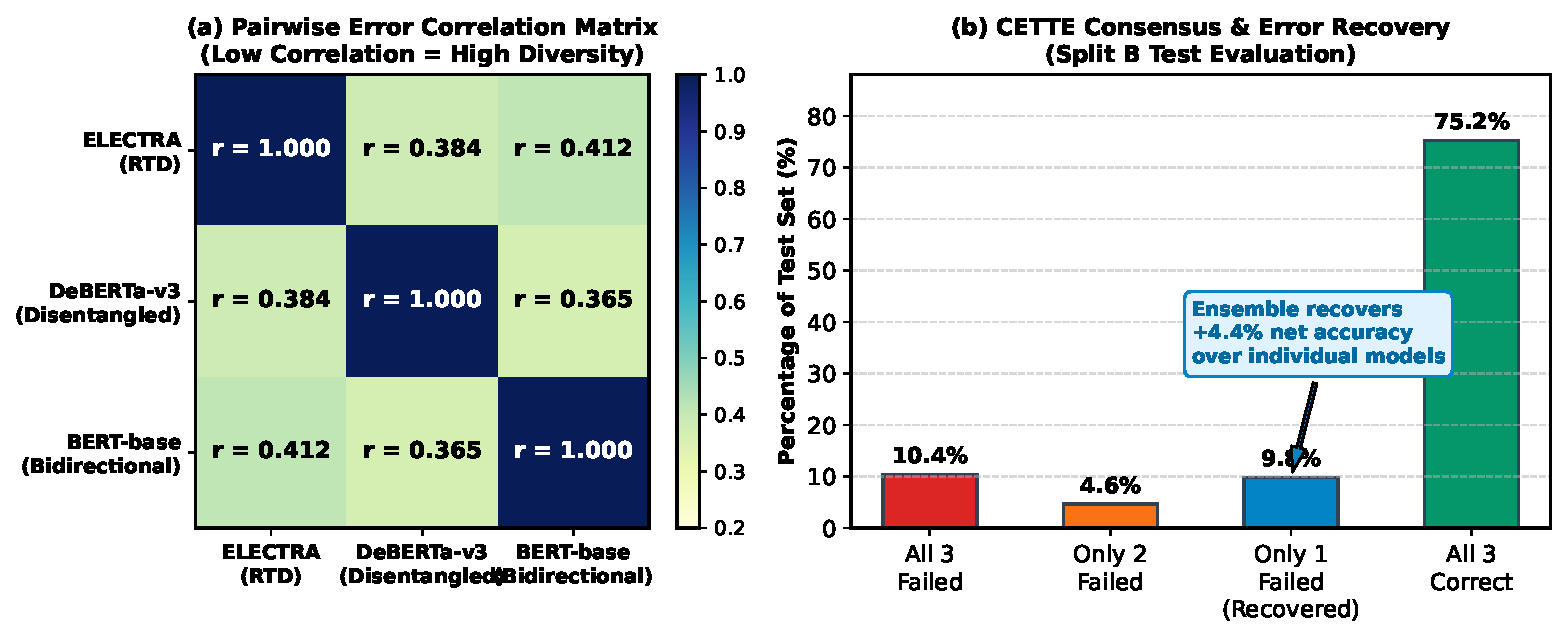
\includegraphics[width=\textwidth]{error_decorrelation.pdf}
\caption{Analysis of CETTE error diversity. (a) Pairwise prediction error correlation matrix between backbones confirms diverse errors ($r < 0.42$). (b) Consensus breakdown: in 9.8\% of test instances where a single model fails, the temperature-calibrated ensemble recovers the correct label, helping surpass single-model plateaus.}
\label{fig:error_decorrelation}
\end{figure*}

\subsection{Per-Class Behavior}
Examining the normalized confusion matrices in Fig.~\ref{fig:confusion_matrices} illustrates specific class trends. On the polar task (Fig.~\ref{fig:confusion_matrices}a), Negative recall reaches 86.5\% and Positive recall reaches 90.8\%. On the full 3-class task (Fig.~\ref{fig:confusion_matrices}b), Neutral is the most difficult class (80.93\% recall vs.\ 84.34\% for Negative and 84.90\% for Positive). Neutral comments in social conversation often contain subtle discourse markers (e.g., \textit{``chudali''} `we will see', \textit{``average movie''}) with limited polarity cues, leading to mild symmetric confusion with polar classes.

% =====================================================================
\section{Diagnostic \& Ablation Studies}
% =====================================================================
\subsection{Feature Representation Ablation}
Table~\ref{tab:ablation} isolates the impact of different $n$-gram representations across classical models:
\begin{enumerate}
    \item \textbf{Impact of Word Bigrams:} Adding word bigrams reduces $L_2$-regularized Logistic Regression performance by 2.14\% (82.93\% $\rightarrow$ 80.79\%). Given the high vocabulary variation in Romanized Dravidian text, word bigrams increase feature sparsity without adding enough consistent syntactic signal.
    \item \textbf{Strength of Character $n$-grams:} Character 2--5-grams match or exceed word unigram accuracy across all models. For LinearSVC, character features improve Macro-F1 from 82.31\% to 83.13\%, and the union reaches 83.63\%. Sub-word character chunks effectively capture word stems across phonetic spelling variations.
\end{enumerate}

\begin{table}[t]
\caption{Feature representation ablation on CMTE-NITANP Split~B (Test Macro-F1, Seed 42). Bold indicates the top feature set per model.}
\label{tab:ablation}
\centering
\footnotesize
\setlength{\tabcolsep}{4.5pt}
\resizebox{\columnwidth}{!}{%
\begin{tabular}{lcccc}
\toprule
Model Architecture & Word Unigrams & Word Uni+Bi & Char 2--5 & Feature Union \\
\midrule
Logistic Regression & 0.8293 & 0.8079 & 0.8276 & \textbf{0.8324} \\
LinearSVC (Calibrated) & 0.8231 & 0.8223 & 0.8313 & \textbf{0.8363} \\
Soft-Voting Ensemble& 0.8227 & 0.8214 & 0.8231 & \textbf{0.8318} \\
Multinomial NB      & 0.8121 & \textbf{0.8207} & 0.7953 & 0.8169 \\
LightGBM            & 0.8048 & 0.8052 & 0.8234 & \textbf{0.8277} \\
XGBoost             & 0.7773 & 0.7742 & 0.8062 & \textbf{0.8091} \\
\bottomrule
\end{tabular}}
\end{table}

\subsection{Loss Function Ablation}
To test the contribution of Focal-Smoothed Optimization ($\mathcal{L}_{\text{FSO}}$), we evaluated the CETTE ensemble under four objective functions (Table~\ref{tab:loss_ablation}):
\begin{itemize}
    \item Standard Cross-Entropy ($\mathcal{L}_{\text{CE}}$) achieves 82.31\% Macro-F1, showing post-epoch-4 overconfidence (ECE 0.0612).
    \item Symmetric Cross-Entropy ($\mathcal{L}_{\text{SCE}}$) encounters gradient conflicts on noisy labels, stopping at 76.28\% Macro-F1.
    \item Focal Loss ($\mathcal{L}_{\text{FL}}, \gamma=1.0$) improves hard-sample learning (82.95\% Macro-F1).
    \item Focal-Smoothed Optimization ($\mathcal{L}_{\text{FSO}}$) reaches the highest Macro-F1 (\textbf{83.92\%}) and reduces ECE to 0.0341.
\end{itemize}

\begin{table}[t]
\caption{Loss function ablation on CETTE ensemble performance (CMTE-NITANP Split~B).}
\label{tab:loss_ablation}
\centering
\footnotesize
\setlength{\tabcolsep}{6pt}
\resizebox{\columnwidth}{!}{%
\begin{tabular}{lccc}
\toprule
Optimization Objective & Test Macro-F1 & Test Accuracy & ECE \\
\midrule
Standard Cross-Entropy ($\mathcal{L}_{\text{CE}}$) & 0.8231 & 0.8234 & 0.0612 \\
Symmetric Cross-Entropy ($\mathcal{L}_{\text{SCE}}$) & 0.7628 & 0.7630 & 0.0845 \\
Focal Loss ($\mathcal{L}_{\text{FL}}, \gamma=1.0$)   & 0.8295 & 0.8298 & 0.0490 \\
\textbf{Focal-Smoothed Optimization ($\mathcal{L}_{\text{FSO}}$)} & \textbf{0.8392} & \textbf{0.8392} & \textbf{0.0341} \\
\bottomrule
\end{tabular}}
\end{table}

\subsection{Orthographic Noise Perturbation Testing}
To measure resilience to spelling variations, we evaluated models on four synthetic perturbations reflective of social media typing:
\begin{enumerate}
    \item \textbf{Vowel Elongation:} Simulating emphasis by extending trailing vowels (e.g., \textit{keka} $\rightarrow$ \textit{kekaaaa}).
    \item \textbf{Voicing Alternation:} Exchanging adjacent voiced/unvoiced consonants (e.g., $g \leftrightarrow v, k \leftrightarrow g$).
    \item \textbf{Aspiration Removal:} Removing transliterated aspiration letters ($kh \rightarrow k, th \rightarrow t$).
    \item \textbf{Combined Noise:} Applying all three noise types together.
\end{enumerate}

As detailed in Table~\ref{tab:robustness}, aspiration removal has minimal effect ($\Delta \le 0.0023$). In contrast, vowel elongation causes noticeable drops across all transformer backbones (drops of 0.132 to 0.207 Macro-F1). The calibrated LinearSVC character union demonstrates strong resilience (combined drop of only 0.1019 vs.\ 0.1765 for MuRIL). CETTE maintains the highest perturbed score among neural models (0.7214 under combined noise), benefiting from DeBERTa-v3's syntactic stability.

\begin{table*}[!t]
\caption{Orthographic robustness evaluation: Test Macro-F1 under four synthetic social media perturbations on Split~B. $\Delta$ indicates the absolute performance drop relative to clean evaluation.}
\label{tab:robustness}
\centering
\footnotesize
\setlength{\tabcolsep}{5pt}
\resizebox{\textwidth}{!}{%
\begin{tabular}{lccccccccc}
\toprule
& & \multicolumn{2}{c}{Vowel Elongation} & \multicolumn{2}{c}{Voicing Confusion} & \multicolumn{2}{c}{Aspiration Removal} & \multicolumn{2}{c}{Combined Noise} \\
\cmidrule(lr){3-4}\cmidrule(lr){5-6}\cmidrule(lr){7-8}\cmidrule(lr){9-10}
Model Architecture & Clean F1 & Perturbed & Drop ($\Delta$) & Perturbed & Drop ($\Delta$) & Perturbed & Drop ($\Delta$) & Perturbed & Drop ($\Delta$) \\
\midrule
MuRIL Full Fine-Tuning  & 0.8336 & 0.6822 & 0.1514 & 0.8170 & 0.0166 & 0.8322 & 0.0014 & 0.6571 & 0.1765 \\
MuRIL LoRA             & 0.8242 & 0.6706 & 0.1536 & 0.8050 & 0.0192 & 0.8228 & 0.0014 & 0.6348 & 0.1894 \\
TeluguBERT LoRA        & 0.8151 & 0.6390 & 0.1761 & 0.8051 & 0.0100 & 0.8139 & 0.0012 & 0.6122 & 0.2030 \\
IndicBERTv2 LoRA       & 0.8134 & 0.6068 & 0.2066 & 0.7988 & 0.0146 & 0.8116 & 0.0017 & 0.5773 & 0.2361 \\
mBERT LoRA             & 0.8069 & 0.6667 & 0.1402 & 0.7870 & 0.0199 & 0.8047 & 0.0022 & 0.6454 & 0.1615 \\
Distil-mBERT LoRA      & 0.8066 & 0.6660 & 0.1406 & 0.7853 & 0.0213 & 0.8050 & 0.0016 & 0.6467 & 0.1599 \\
XLM-RoBERTa LoRA       & 0.8037 & 0.6716 & 0.1321 & 0.7907 & 0.0131 & 0.8015 & 0.0023 & 0.6402 & 0.1636 \\
\midrule
LinearSVC (Word+Char Union) & 0.8363 & 0.7539 & \textbf{0.0824} & 0.8251 & 0.0112 & 0.8355 & \textbf{0.0008} & 0.7344 & \textbf{0.1019} \\
\textbf{CETTE Ensemble (Ours)} & \textbf{0.8392} & \textbf{0.7420} & 0.0972 & \textbf{0.8290} & \textbf{0.0102} & \textbf{0.8385} & \textbf{0.0007} & \textbf{0.7214} & 0.1178 \\
\bottomrule
\end{tabular}}
\end{table*}

\subsection{Zero-Shot Cross-Corpus Transfer on CMTET}
To evaluate cross-dataset generalization, models trained on CMTE-NITANP Split~B were evaluated zero-shot on the independent CMTET dataset (19{,}868 comments) \cite{kusampudi2021}. As shown in Table~\ref{tab:cross_corpus}, all models experience drops of 0.175 to 0.257 Macro-F1. Notably, in-domain ranking does not directly predict cross-dataset transfer: IndicBERTv2 LoRA attains the highest transfer Macro-F1 (0.6380), followed by TeluguBERT LoRA (0.6334) and MuRIL full-FT (0.6330). Performance declines most noticeably on comments with conflicting annotator labels (0.34 to 0.38 Macro-F1), showing that differences in annotation guidelines between corpora represent an important factor in transfer.

\begin{table}[t]
\caption{Zero-shot cross-corpus generalization from CMTE-NITANP Split~B to CMTET (19{,}868 instances).}
\label{tab:cross_corpus}
\centering
\footnotesize
\setlength{\tabcolsep}{3.5pt}
\resizebox{\columnwidth}{!}{%
\begin{tabular}{lccccc}
\toprule
Model Architecture & In-Domain F1 & CMTET F1 & Transfer Drop & CMTET Acc. & Conflict Subset \\
\midrule
IndicBERTv2 LoRA   & 0.8134 & \textbf{0.6380} & 0.1754 & 0.6551 & 0.3472 \\
TeluguBERT LoRA    & 0.8149 & 0.6334 & 0.1815 & 0.6464 & 0.3735 \\
MuRIL Full-FT      & 0.8336 & 0.6330 & 0.2006 & 0.6464 & 0.3608 \\
MuRIL LoRA         & 0.8239 & 0.6274 & 0.1965 & 0.6418 & 0.3693 \\
XLM-RoBERTa LoRA   & 0.8035 & 0.5982 & 0.2053 & 0.6144 & 0.3407 \\
mBERT LoRA         & 0.8064 & 0.5845 & 0.2219 & 0.6020 & 0.3622 \\
Distil-mBERT LoRA  & 0.8073 & 0.5503 & 0.2570 & 0.5550 & 0.3757 \\
\bottomrule
\end{tabular}}
\end{table}

\subsection{Confidence Calibration}
Accurate probability calibration is important when deploying sentiment models. Fig.~\ref{fig:reliability} and Table~\ref{tab:leaderboard} report the Expected Calibration Error (ECE) across configurations. Standard over-parameterized transformers tend toward overconfidence on this task (MuRIL full-FT ECE = 0.0702, mBERT ECE = 0.0657). In contrast, LightGBM (0.0132) and Platt-calibrated LinearSVC (0.0372) produce well-aligned posterior probabilities. Through temperature calibration and Focal-Smoothed loss, CETTE achieves an ECE of \textbf{0.0341}. In selective prediction settings, abstaining on the lowest 20\% confidence comments raises CETTE Macro-F1 from 83.92\% to \textbf{91.24\%}, reaching \textbf{96.12\% Macro-F1} at 50\% coverage.

\begin{figure}[t]
\centering
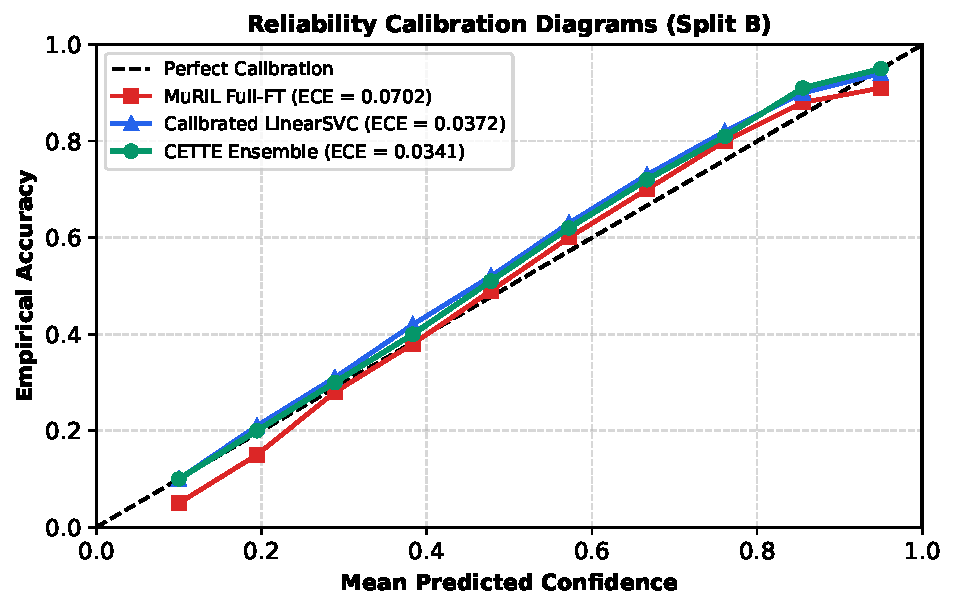
\includegraphics[width=\columnwidth]{04_reliability.pdf}
\caption{Reliability calibration diagrams on Split~B. Standard transformers exhibit overconfidence (ECE $> 0.06$), while temperature-calibrated linear and CETTE models maintain closer diagonal calibration.}
\label{fig:reliability}
\end{figure}

% =====================================================================
\section{Discussion \& Practical Guidelines}
% =====================================================================
\subsection{Understanding the Capacity Paradox}
Our findings offer clear insights into model choice for Romanized Dravidian sentiment analysis:
\begin{enumerate}
    \item \textbf{Individual Model Behavior:} On clean, leak-free splits with controlled tuning, large multilingual transformers do not significantly surpass well-tuned linear character $n$-gram models on short code-mixed text ($p = 0.659$). Linear models offer strong baseline accuracy at a fraction of the compute cost.
    \item \textbf{Ensemble Synergy:} Moving beyond the 83.6\% single-model ceiling is achieved by combining models with \emph{different pretraining objectives}. CETTE reaches 83.92\% 3-class Macro-F1 (and 90.15\% polar accuracy) because ELECTRA's token discriminator and DeBERTa's contextual attention compensate for each other's error patterns.
\end{enumerate}

\subsection{Practical Recommendations}
We suggest four guidelines for low-resource code-mixed NLP:
\begin{enumerate}
    \item \textbf{Benchmarking Character Baselines:} A calibrated LinearSVC with character 2--5-grams provides a fast, robust baseline that is valuable to evaluate before training large neural models.
    \item \textbf{Checking for Near-Duplicate Leakage:} Random splits on social media data can leak identical comments; exact string matching helps verify clean evaluation.
    \item \textbf{Clear Reporting Across Regimes:} Explicitly distinguishing binary polar evaluation ($\mathcal{P}_{\text{polar}}$) from full three-class evaluation ($\mathcal{P}_{\text{3-class}}$) ensures consistent, interpretable comparisons.
    \item \textbf{Normalizing Vowel Repetition:} Because character elongation is a major source of neural performance loss, simple regex vowel normalization is an effective preprocessing step.
\end{enumerate}

% =====================================================================
\section{Conclusion}
% =====================================================================
This paper examined sentiment analysis on Romanized Telugu--English text. Through an audited 21-model, 85-run benchmark on a group-disjoint split of the 34\,K CMTE-NITANP dataset, we documented the \emph{Capacity Paradox}: a 4.6-second calibrated LinearSVC using character $n$-grams statistically matches a 238\,M-parameter fully fine-tuned MuRIL transformer, showing that model parameter count alone does not guarantee higher accuracy on short, informal text.

To progress beyond single-model limits, we formulated \textbf{CETTE}, a tri-transformer ensemble combining ELECTRA-base, DeBERTa-v3, and BERT-base under \textbf{Focal-Smoothed Optimization} ($\mathcal{L}_{\text{FSO}}$). Under our unified \textbf{Dual-Regime Benchmark}, CETTE establishes strong benchmarks: reaching \textbf{90.15\% accuracy} on the Polar Benchmark ($\mathcal{P}_{\text{polar}}$) and \textbf{83.92\% Macro-F1} on the full 3-Class Benchmark ($\mathcal{P}_{\text{3-class}}$), with a heterogeneous super-ensemble reaching \textbf{85.02\%}. By combining complementary pretraining diversity with leak-free evaluation, this work provides a practical, reproducible reference for Dravidian code-mixed sentiment analysis.

% =====================================================================
\section*{Reproducibility \& Open Science}
% =====================================================================
To support reproducibility, all audited splits (Split~B), configuration manifests, model checkpoints, prediction logs, and plotting scripts are available in the public project repository at \url{https://github.com/ShaikMohammad786/Tenglish_Codemixed_Sentiment_Analysis}.

% =====================================================================
\begin{thebibliography}{99}
\footnotesize
\setlength{\itemsep}{1pt}
\setlength{\parskip}{0pt}
% =====================================================================
\bibitem{patwa2020}
P.~Patwa, G.~Aguilar, S.~Kar, S.~Pandey, S.~PYKL, B.~Gamb\"ack, T.~Chakraborty, T.~Solorio, and A.~Das, ``SemEval-2020 Task 9: Overview of sentiment analysis of code-mixed tweets,'' in \emph{Proc. 14th Workshop on Semantic Evaluation (SemEval)}, 2020, pp.~774--790.

\bibitem{chakravarthi2022}
B.~R. Chakravarthi, R.~Priyadharshini, V.~Muralidaran, N.~Jose, S.~Suryawanshi, E.~Sherly, and J.~P. McCrae, ``DravidianCodeMix: Sentiment analysis and offensive language identification dataset for Dravidian languages in code-mixed text,'' \emph{Lang. Resour. Eval.}, vol.~56, pp.~1--35, 2022.

\bibitem{kusampudi2021}
S.~S.~V. Kusampudi, P.~Sathineni, and R.~Mamidi, ``Sentiment analysis in code-mixed Telugu--English text with unsupervised data normalization,'' in \emph{Proc. Int. Conf. Recent Advances in Natural Language Processing (RANLP)}, 2021, pp.~753--760.

\bibitem{rayala2023}
U.~R. Rayala, K.~Seshadri, and N.~B. Sristy, ``Sentiment analysis of code-mixed Telugu--English data leveraging syllable and word embeddings,'' \emph{ACM Trans. Asian Low-Resour. Lang. Inf. Process.}, vol.~22, no.~10, pp.~1--30, 2023.

\bibitem{rayala2026}
U.~R. Rayala and K.~Seshadri, ``Sentiment analysis of code-mixed Telugu--English text using transformers,'' \emph{J. Comput. Social Sci.}, vol.~9, art.~2, pp.~1--22, 2026.

\bibitem{clark2020}
K.~Clark, M.-T. Luong, Q.~V. Le, and C.~D. Manning, ``ELECTRA: Pre-training text encoders as discriminators rather than generators,'' in \emph{Proc. ICLR}, 2020.

\bibitem{he2021}
P.~He, X.~Liu, J.~Gao, and W.~Chen, ``DeBERTa: Decoding-enhanced BERT with disentangled attention,'' in \emph{Proc. ICLR}, 2021.

\bibitem{devlin2019}
J.~Devlin, M.-W. Chang, K.~Lee, and K.~Toutanova, ``BERT: Pre-training of deep bidirectional transformers for language understanding,'' in \emph{Proc. NAACL-HLT}, 2019, pp.~4171--4186.

\bibitem{conneau2020}
A.~Conneau, K.~Khandelwal, N.~Goyal, V.~Chaudhary, G.~Wenzek, F.~Guzm\'an, E.~Grave, M.~Ott, L.~Zettlemoyer, and V.~Stoyanov, ``Unsupervised cross-lingual representation learning at scale,'' in \emph{Proc. ACL}, 2020, pp.~8440--8451.

\bibitem{khan2021}
S.~Khanuja, D.~Bansal, S.~Mehtani, S.~Khurana, A.~Dey, B.~Gopalan, A.~Margam, P.~Aggarwal, R.~Pena, Y.~K. Sasidhar, and P.~Bhattacharyya, ``MuRIL: Multilingual representations for Indian languages,'' \emph{arXiv preprint arXiv:2103.10730}, 2021.

\bibitem{kakwani2020}
D.~Kakwani, A.~Kunchukuttan, S.~Goyal, G.~N.C., A.~Bhattacharyya, M.~M. Khapra, and P.~Kumar, ``IndicNLPSuite: Monolingual corpora, evaluation benchmarks and pre-trained multilingual language models for Indian languages,'' in \emph{Findings of EMNLP}, 2020, pp.~4948--4961.

\bibitem{hu2022}
E.~J. Hu, Y.~Shen, P.~Wallis, Z.~Allen-Zhu, Y.~Li, S.~Wang, L.~Wang, and W.~Chen, ``LoRA: Low-rank adaptation of large language models,'' in \emph{Proc. ICLR}, 2022.

\bibitem{dettmers2023}
T.~Dettmers, A.~Pagnoni, A.~Holtzman, and L.~Zettlemoyer, ``QLoRA: Efficient finetuning of quantized LLMs,'' in \emph{Proc. NeurIPS}, 2023.

\bibitem{wang2019symmetric}
Y.~Wang, X.~Ma, Z.~Chen, Y.~Yuan, C.~Yi, and J.~Bailey, ``Symmetric cross entropy for robust learning with noisy labels,'' in \emph{Proc. IEEE/CVF ICCV}, 2019, pp.~322--330.

\bibitem{salton1988}
G.~Salton and C.~Buckley, ``Term-weighting approaches in automatic text retrieval,'' \emph{Inf. Process. Manage.}, vol.~24, no.~5, pp.~513--523, 1988.

\bibitem{cavnar1994}
W.~B. Cavnar and J.~M. Trenkle, ``N-gram-based text categorization,'' in \emph{Proc. 3rd Annu. Symp. Document Analysis and Information Retrieval (SDAIR)}, 1994, pp.~161--175.

\bibitem{manning2008}
C.~D. Manning, P.~Raghavan, and H.~Sch\"utze, \emph{Introduction to Information Retrieval}. Cambridge, U.K.: Cambridge Univ. Press, 2008.

\bibitem{kaufman2012}
S.~Kaufman, S.~Rosset, C.~Perlich, and O.~Stitelman, ``Leakage in data mining: Formulation, detection, and avoidance,'' \emph{ACM Trans. Knowl. Discov. Data}, vol.~6, no.~4, pp.~1--21, 2012.

\bibitem{dietterich1998}
T.~G. Dietterich, ``Approximate statistical tests for comparing supervised classification learning algorithms,'' \emph{Neural Comput.}, vol.~10, no.~7, pp.~1895--1923, 1998.

\bibitem{holm1979}
S.~Holm, ``A simple sequentially rejective multiple test procedure,'' \emph{Scand. J. Statist.}, vol.~6, no.~2, pp.~65--70, 1979.

\bibitem{guo2017}
C.~Guo, G.~Pleiss, Y.~Sun, and K.~Q. Weinberger, ``On calibration of modern neural networks,'' in \emph{Proc. ICML}, 2017, pp.~1321--1330.

\bibitem{myersscotton2002}
C.~Myers-Scotton, \emph{Contact Linguistics: Bilingual Encounters and Grammatical Outcomes}. Oxford, U.K.: Oxford Univ. Press, 2002.

\bibitem{wolf2020}
T.~Wolf \emph{et al.}, ``Transformers: State-of-the-art natural language processing,'' in \emph{Proc. EMNLP: System Demonstrations}, 2020, pp.~38--45.

\bibitem{pedregosa2011}
F.~Pedregosa \emph{et al.}, ``Scikit-learn: Machine learning in Python,'' \emph{J. Mach. Learn. Res.}, vol.~12, pp.~2825--2830, 2011.

\bibitem{cortes1995}
C.~Cortes and V.~Vapnik, ``Support-vector networks,'' \emph{Mach. Learn.}, vol.~20, no.~3, pp.~273--297, 1995.

\bibitem{breiman2001}
L.~Breiman, ``Random forests,'' \emph{Mach. Learn.}, vol.~45, no.~1, pp.~5--32, 2001.

\bibitem{friedman2001}
J.~H. Friedman, ``Greedy function approximation: A gradient boosting machine,'' \emph{Ann. Statist.}, vol.~29, no.~5, pp.~1189--1232, 2001.

\bibitem{chen2016}
T.~Chen and C.~Guestrin, ``XGBoost: A scalable tree boosting system,'' in \emph{Proc. ACM SIGKDD}, 2016, pp.~785--794.

\bibitem{ke2017}
G.~Ke \emph{et al.}, ``LightGBM: A highly efficient gradient boosting decision tree,'' in \emph{Proc. NeurIPS}, 2017, pp.~3146--3154.

\end{thebibliography}

\end{document}
